% !TeX root = ../FoodSpy.tex
% \section{Utilizarea aplicației}

\section{Procesul de înregistrare și autentificare}
La momentul deschiderii aplicației, utilizatorul este întâmpinat direct cu formularul HTML în care trebuie să introducă un e-mail, o parolă și un obiectiv caloric de atins. Formularul de înregistrare, completat, este ilustrat în (Fig. \ref{fig:71}). Dacă are deja cont, utilizatorul trebuie să apese pe butonul ”Already have an account? Log in”. La apăsarea butonului, din formular dispare câmpul ”Target calories”, după cum se poate observa în (Fig. \ref{fig:72}).

\begin{figure}[!htb]
	\centering
	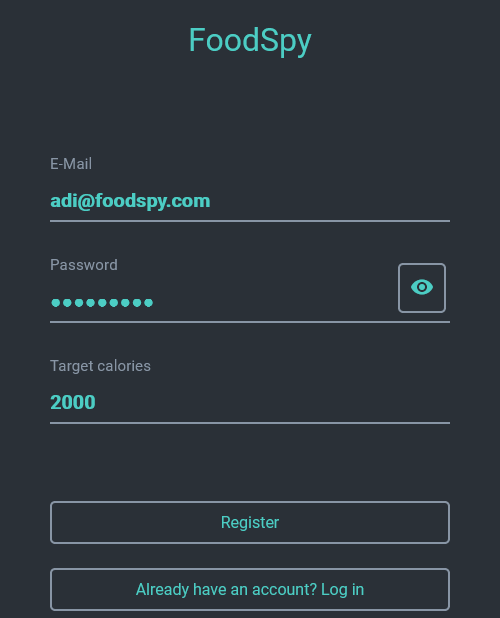
\includegraphics[width=0.5\textwidth]
	{../LaTeX/Images/App/auth_register.PNG}
	\caption{Pagina principală a aplicației}
	\label{fig:71}
\end{figure}

\begin{figure}[!htb]
	\centering
	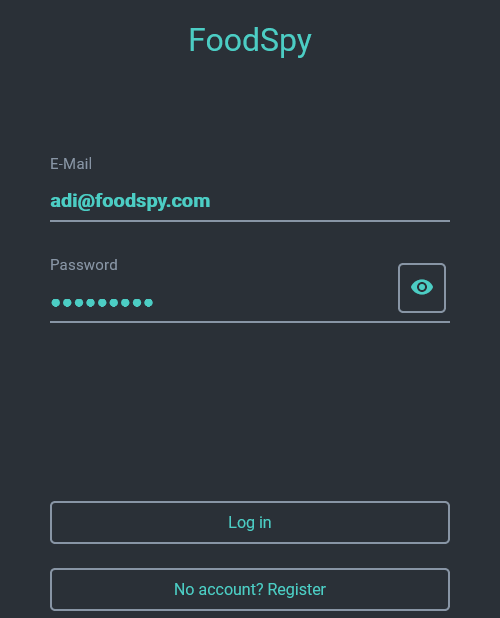
\includegraphics[width=0.5\textwidth]
	{../LaTeX/Images/App/auth_login.PNG}
	\caption{Formularul de autentificare}
	\label{fig:72}
\end{figure}

”adi@foodspy.com” nu este o adresă de mail persistată în baza de date. În acest caz, clientul trimite mesajul ”No account found!” (Fig. \ref{fig:73}) deasupra formularului pentru a înștiința utilizatorul că înainte de a accesa aplicația, trebuie mai întâi să-și creeze un cont.

\begin{figure}[!htb]
	\centering
	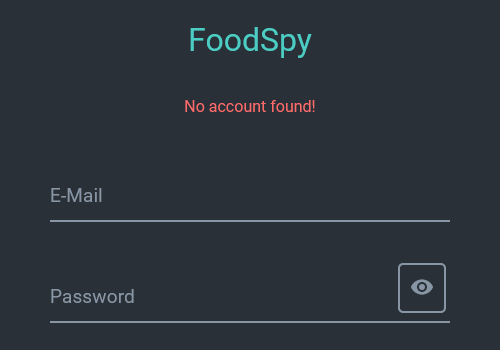
\includegraphics[width=0.5\textwidth]
	{../LaTeX/Images/App/auth_login_no-account.PNG}
	\caption{Eroarea afișată în cazul unui cont inexistent}
	\label{fig:73}
\end{figure}

După înregistrarea cu aceeași adresă de e-mail care a generat eroarea din (Fig. \ref{fig:73}) (”adi@foodspy.com”), clientul trimite un mesaj de informare și anume ”Account created! You can log in now!”.


\section{Adăugarea unui aliment la o masă}
După procesul de autentificare, utilizatorul este redirecționat la tabloul de bord al aplicației, ilustrat în (Fig. \ref{fig:74}).

\begin{figure}[!htb]
	\centering
	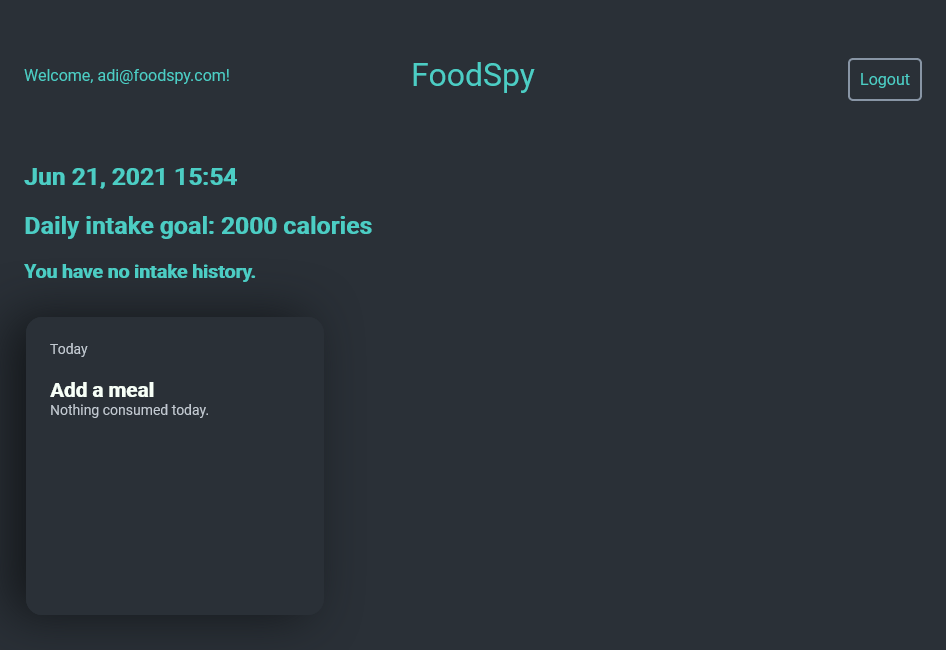
\includegraphics[width=0.9\textwidth]
	{../LaTeX/Images/App/dashboard.PNG}
	\caption{Tabloul de bord al aplicației}
	\label{fig:74}
\end{figure}

În dashboard (”tabloul de bord”), clientul afișează adresa de e-mail a utilizatorului autentificat, obiectivul caloric propus și data de astăzi. După cum se observă în (Fig. \ref{fig:74}), pentru această adresă de e-mail nu există nicio intrare în jurnalul aportului zilnic de calorii, deci clientul afișează ”You have no intake history” și ”Nothing consumed today”.
\\ \\
Dacă utilizatorul dorește să adauge o masă în jurnal, trebuie să acceseze pagina ”AddMeal” prin hyperlink-ul denumit ”Add a meal”, care se colorează în turcoaz la evenimentul de hover al mouse-ului, ilustrat în (Fig. \ref{fig:75}).

\begin{figure}[!htb]
	\centering
	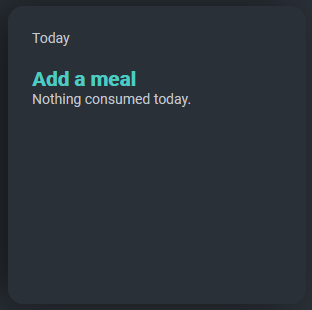
\includegraphics[width=0.5\textwidth]
	{../LaTeX/Images/App/dashboard_add.PNG}
	\caption{Hyperlink pentru adăugarea unei mese}
	\label{fig:75}
\end{figure}

Odată accesată pagina ”AddMeal” (Fig. \ref{fig:76}), utilizatorul poate căuta alimente în baza de date prin bara de căutare, care are un placeholder (”Look for food...”) pus pe elementul ”<input>”.
\\ \\
Bara de căutare execută un request către API doar în momentul în care au fost introduse nume de alimente de cel puțin 3 caractere în lungime. De asemenea, nu este nevoie ca utilizatorul să execute manual operațiunea de filtrare a alimentelor, deoarece clientul inițiază căutarea în baza de date, când termenul de căutare este valid.

\begin{figure}[!htb]
	\centering
	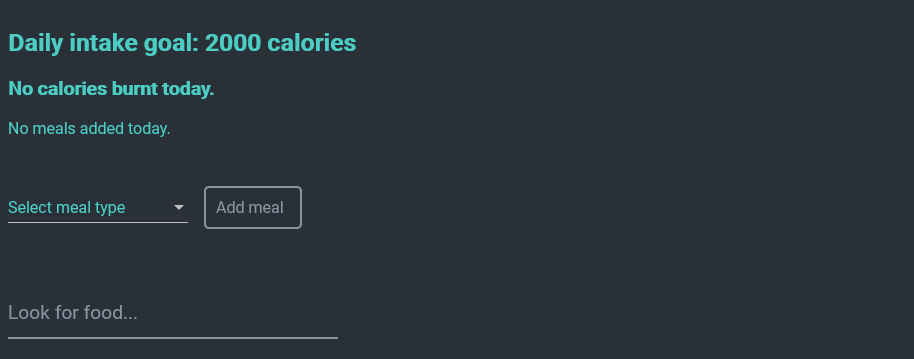
\includegraphics[width=0.8\textwidth]
	{../LaTeX/Images/App/add.PNG}
	\caption{Pagina ”AddMeal”}
	\label{fig:76}
\end{figure}

Utilizatorul caută după termenul ”magiun”, se face un request către interfața de programare care se ocupă de gestiunea aportului zilnic de calorii. Interfața întoarce lista de rezultate, în acest caz, alimentul cu numele ”Magiun de prune Cămara Noastră” (Fig. \ref{fig:77}).

\begin{figure}[!htb]
	\centering
	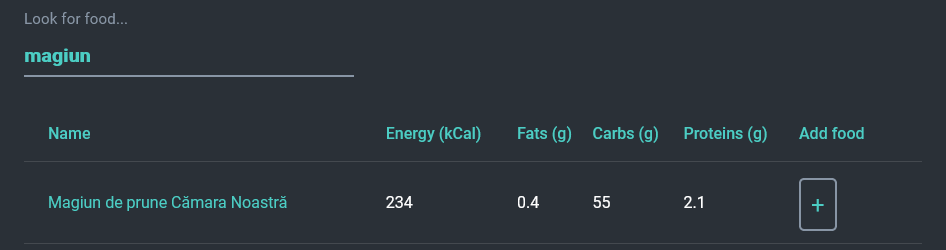
\includegraphics[width=0.8\textwidth]
	{../LaTeX/Images/App/add_magiun.PNG}
	\caption{Lista de rezultate a căutării}
	\label{fig:77}
\end{figure}

\begin{figure}[!htb]
	\centering
	
\includegraphics[width=0.5\textwidth]
	{../LaTeX/Images/App/add_gem.PNG}
	\caption{Lista de rezultate este goală}
	\label{fig:78}
\end{figure}

Dacă lista de rezultate este o listă goală, înseamnă că alimentul nu se află în baza de date și se afișează utilizatorului mesajul ”No matching foods found.”, după cum este ilustrat în (Fig. \ref{fig:77}).
\\ \\
Despre alimentul cu numele ”Magiun de prune Cămara Noastră” se afișează în format tabelar o colecție sumară de informații nutriționale și anume ”Energy”, ”Fats”, ”Carbohydrates” și ”Proteins”. Dacă utilizatorul dorește mai multe informații, trebuie să acceseze pagina ”EditFoodDialogue” prin butonul ”+” de sub coloana ”Add food”.
\\ \\
După apăsarea butonului ”+” (Fig. \ref{fig:77}), clientul deschide o căsuță de dialog (Fig. \ref{fig:78}) care afișează lista întreagă de informații nutriționale ale alimentului, împreună cu un formular pe care îl poate completa. Formularul are două câmpuri, unul pentru cantitatea de mâncare, iar celălalt pentru unitatea de măsură a cantității, în acest caz, ”grams”.
\\ \\
Formularul este deja populat cu o valoare default de ”100” pentru cantitate. Dacă utilizatorul nu completează cantitatea sau introduce o cantitate prea mare, un mesaj de eroare este afișat, ilustrat în (Fig. \ref{fig:710}) și (Fig. \ref{fig:711}).

\begin{figure}[!htb]
	\centering
	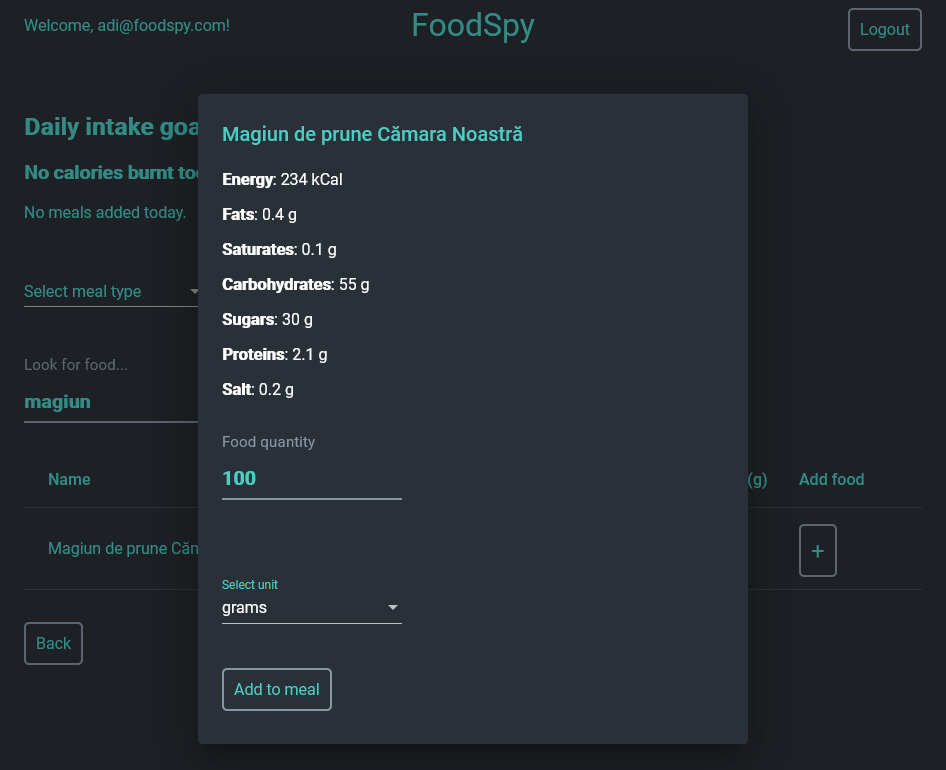
\includegraphics[width=0.8\textwidth]
	{../LaTeX/Images/App/add_edit.PNG}
	\caption{Căsuța de dialog care permite adăugarea alimentului la o masă}
	\label{fig:710}
\end{figure}

\begin{figure}[!htb]
	\centering
	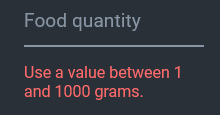
\includegraphics[width=0.25\textwidth]
	{../LaTeX/Images/App/add_edit-error.PNG}
	\caption{Eroare la validarea câmpului ”Food quantity” dacă utilizatorul nu introduce cantitatea}
	\label{fig:711}
\end{figure}

\begin{figure}[!htb]
	\centering
	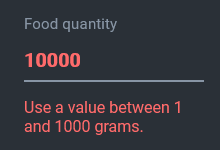
\includegraphics[width=0.25\textwidth]
	{../LaTeX/Images/App/add_edit-error-10000.PNG}
	\caption{Eroare la validarea câmpului ”Food quantity” dacă utilizatorul introduce o cantitate prea mare}
	\label{fig:712}
\end{figure}

Dacă utilizatorul introduce o valoare corespunzătoare pentru cantitate, butonul ”Add to meal” din căsuța de dialog devine activ și se poate astfel adăuga alimentul la masă. Automat, la apăsarea butonului, se populează lista de mese (un ”array”) în clasa TypeScript ”AddMeal”. Singurul pas care mai trebuie făcut este selectarea unuia dintre tipurile de masă acceptat în aplicație (Fig. \ref{fig:713}).

\begin{figure}[!htb]
	\centering
	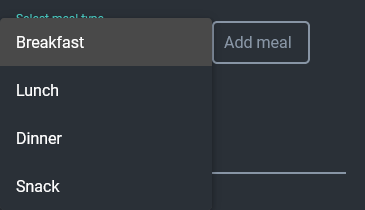
\includegraphics[width=0.5\textwidth]
	{../LaTeX/Images/App/add_meal-type.PNG}
	\caption{Cele 4 tipuri de masă disponibile utilizatorului}
	\label{fig:713}
\end{figure}

Când lista de mese are cel puțin un aliment și utilizatorul a selectat și un tip de masă, butonul ”Add meal” (Fig. \ref{fig:76}) devine activ. La apăsarea butonului, se face un nou request către ”FoodSpyAPI”, se persistă intrarea în jurnal în baza de date și se reîncarcă pagina ”AddMeal” pentru a reflecta ultima stare a jurnalului din ziua respectivă.
\\ \\
Se poate observa că în loc de ”No meals added today” (Fig. \ref{fig:714}), mesajul care apare este ”Today you had one meal” și apare și un buton, ”View”, care permite afișarea în detaliu a mâncărurilor și meselor consumate, până la momentul respectiv în acea zi (Fig. \ref{fig:715}).

\begin{figure}[!htb]
	\centering
	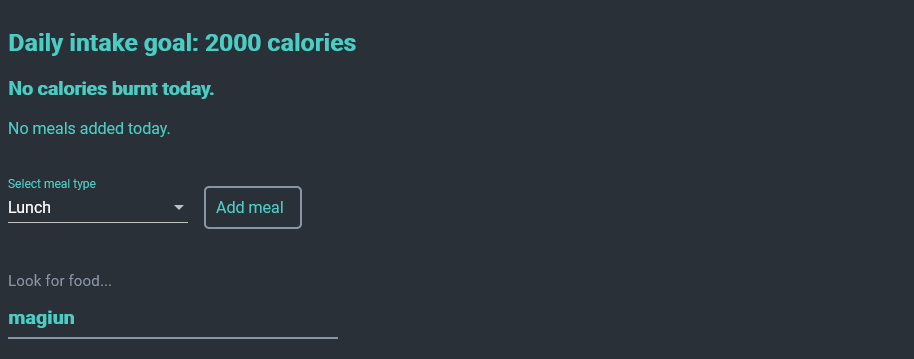
\includegraphics[width=0.7\textwidth]
	{../LaTeX/Images/App/add_lunch.PNG}
	\caption{Adăugarea unei mese de tip ”Lunch”}
	\label{fig:714}
\end{figure}

\begin{figure}[!htb]
	\centering
	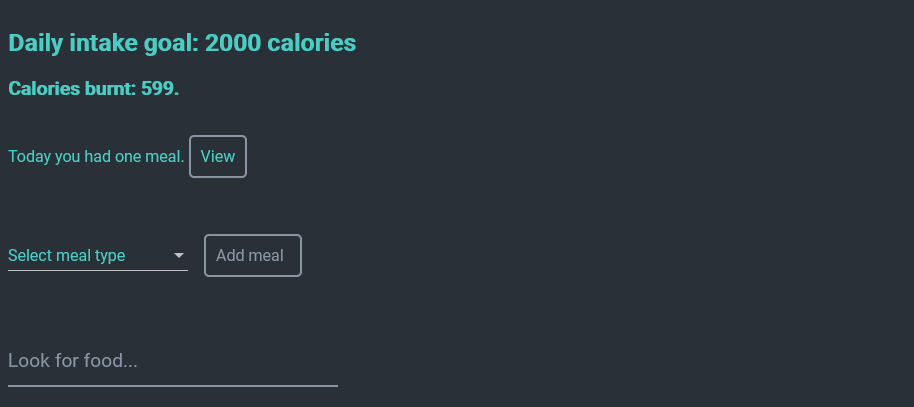
\includegraphics[width=0.7\textwidth]
	{../LaTeX/Images/App/add_lunch-result.PNG}
	\caption{Rezultatul adăugării unei mese de tip ”Lunch”}
	\label{fig:715}
\end{figure}

În timpul zilei, pe măsură ce utilizatorul înregistrează mese în jurnal, mesajul ”Today you had .. meal(s)” va reflecta numărul acestora, până când se atinge numărul maxim de mese care pot fi adăugate, adică 4. Utilizatorul poate adăuga, de exemplu, un aliment sau mai multe la tipul de masă ”Breakfast” sau ”Dinner”, dar nu poate adăuga un alt tip de masă diferit de cele patru permise în aplicație.


\section{Vizualizarea în detaliu a jurnalului}
Dacă utilizatorul apasă butonul de ”View”, acesta este direcționat către pagina ”History” (Fig. \ref{fig:716}).
\\ \\
Aici, se compară caloriile consumate până la momentul respectiv cu numărul de calorii pe care utilizatorul și le-a propus ca obiectiv. Totodată este afișat un procentaj al completării acestui obiectiv printr-o animație și un grafic.
\\ \\
Informațiile nutriționale afișate sub graficul descris mai sus reprezintă totalul grăsimilor, carbohidraților, zaharurilor, șamd., al tuturor mâncărurilor consumate în ziua respectivă.
În acest caz, cantitățile nutriționale sunt raportate la cele 256 de grame de ”Magiun de prune Cămara Noastră” consumate.
\\ \\
Folosind butonul ”Back”, utilizatorul se poate întoarce la tabloul de bord al aplicației.

\begin{figure}[!htb]
	\centering
	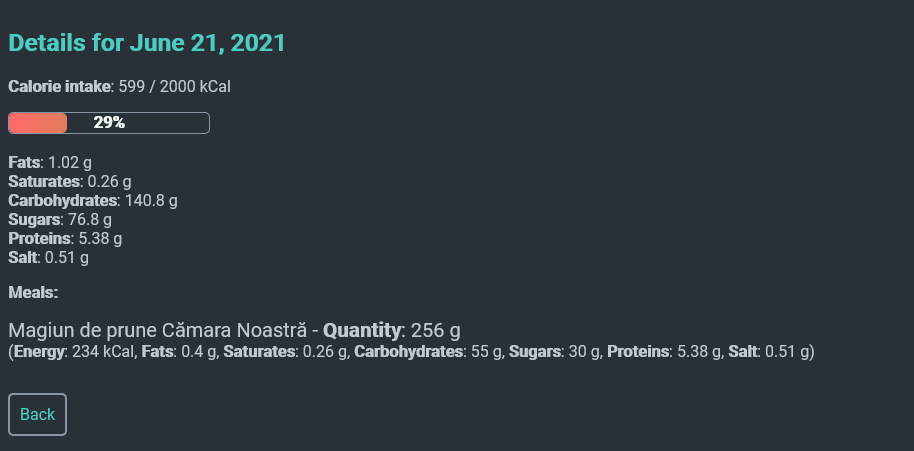
\includegraphics[width=0.9\textwidth]
	{../LaTeX/Images/App/history.PNG}
	\caption{Jurnalul detaliat pentru ziua de 21 iunie}
	\label{fig:716}
\end{figure}


\section{Revenirea la tabloul de bord}
Apăsând butonul ”Back” din pagina ”History”, utilizatorul a revenit la tabloul de bord.

\begin{figure}[!htb]
	\centering
	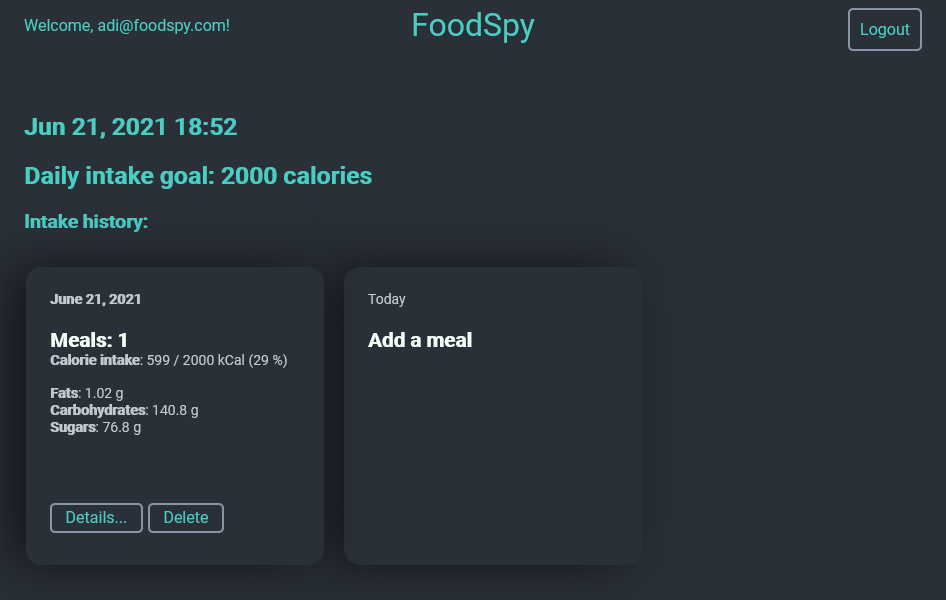
\includegraphics[width=0.9\textwidth]
	{../LaTeX/Images/App/history_result.PNG}
	\caption{Tabloul de bord pentru ziua de 21 iunie}
	\label{fig:717}
\end{figure}

Pe lângă hyperlink-ul care îi permite acestuia să adauge alte mâncăruri (Fig. \ref{fig:75}), există acum o intrare în jurnal pentru ziua curentă, ilustrată în (Fig. \ref{fig:718}). Intrarea este afișată în mod sumar, restul detaliilor fiind conținute în pagina ”History”.

\begin{figure}[!htb]
	\centering
	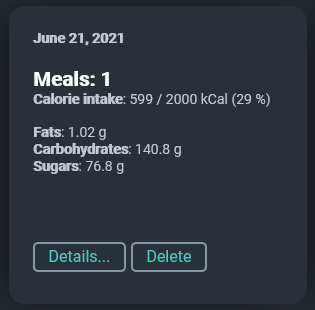
\includegraphics[width=0.5\textwidth]
	{../LaTeX/Images/App/history_today.PNG}
	\caption{Jurnalul sumar al zilei de 21 iunie}
	\label{fig:718}
\end{figure}

Butonul ”Details” trimite utilizatorul către aceeași pagină de ”History” din care a venit, iar butonul de ”Delete” șterge intrarea din ziua respectivă din baza de date.
\\ \\
Utilizatorul se poate deconecta din aplicație prin butonul ”Logout” din colțul din dreapta sus (Fig. \ref{fig:717}).